\documentclass[11pt]{article}
\usepackage{xspace}
\usepackage{palatino}
\usepackage{fancyhdr}
\usepackage{graphicx}
\usepackage[headings]{fullpage}
\pagestyle{fancy}
\newcommand\STex{Simple\TeX\xspace}
\newcommand\LTex{\LaTeX\xspace}
\lhead{\begin{slshape}Justin Bailey\end{slshape}}
\chead{\begin{slshape}\copyright\ 2010 \STex\end{slshape}}
\rhead{\begin{slshape}\today\end{slshape}}
\fancypagestyle{first}{\fancyfoot{}} % No page numbers
\renewcommand\floatpagefraction{0.8} 
\begin{document}
\thispagestyle{first}
\section*{Overview}
The \STex architecture has five components. Some are composed of many servers:
\begin{itemize}
\item \textbf{Web} -- Stateless servers, running (J)Ruby on Rails, for managing application UI. Also handles file upload/download.
\item \textbf{Database} -- Handles user information, document structure, and permissions.
\item \textbf{\LTex Processors} -- Stateless servers responsible for generating PDF documents from \LTex source. As demand increases more servers can be brought online.
\item \textbf{EtherPad Servers} -- Hosts EtherPad instances. As demand increases more can be provisioned.
\item \textbf{Load Listener} -- Monitors load of \LTex and EtherPad servers, and can provision additional servers if needed. Also able to remove servers as load decreases.
\item \textbf{Message Bus} -- Implemented via Simple Queue Service (SQS). All requests for \LTex processing, EtherPad instances, and other as-yet-undetermined resources from the web servers will be mediated by the message bus.
\end{itemize}
\noindent
Figure \ref{fig_arch} shows the relation and responsibilities of these components.

\begin{figure}[h]
\centering
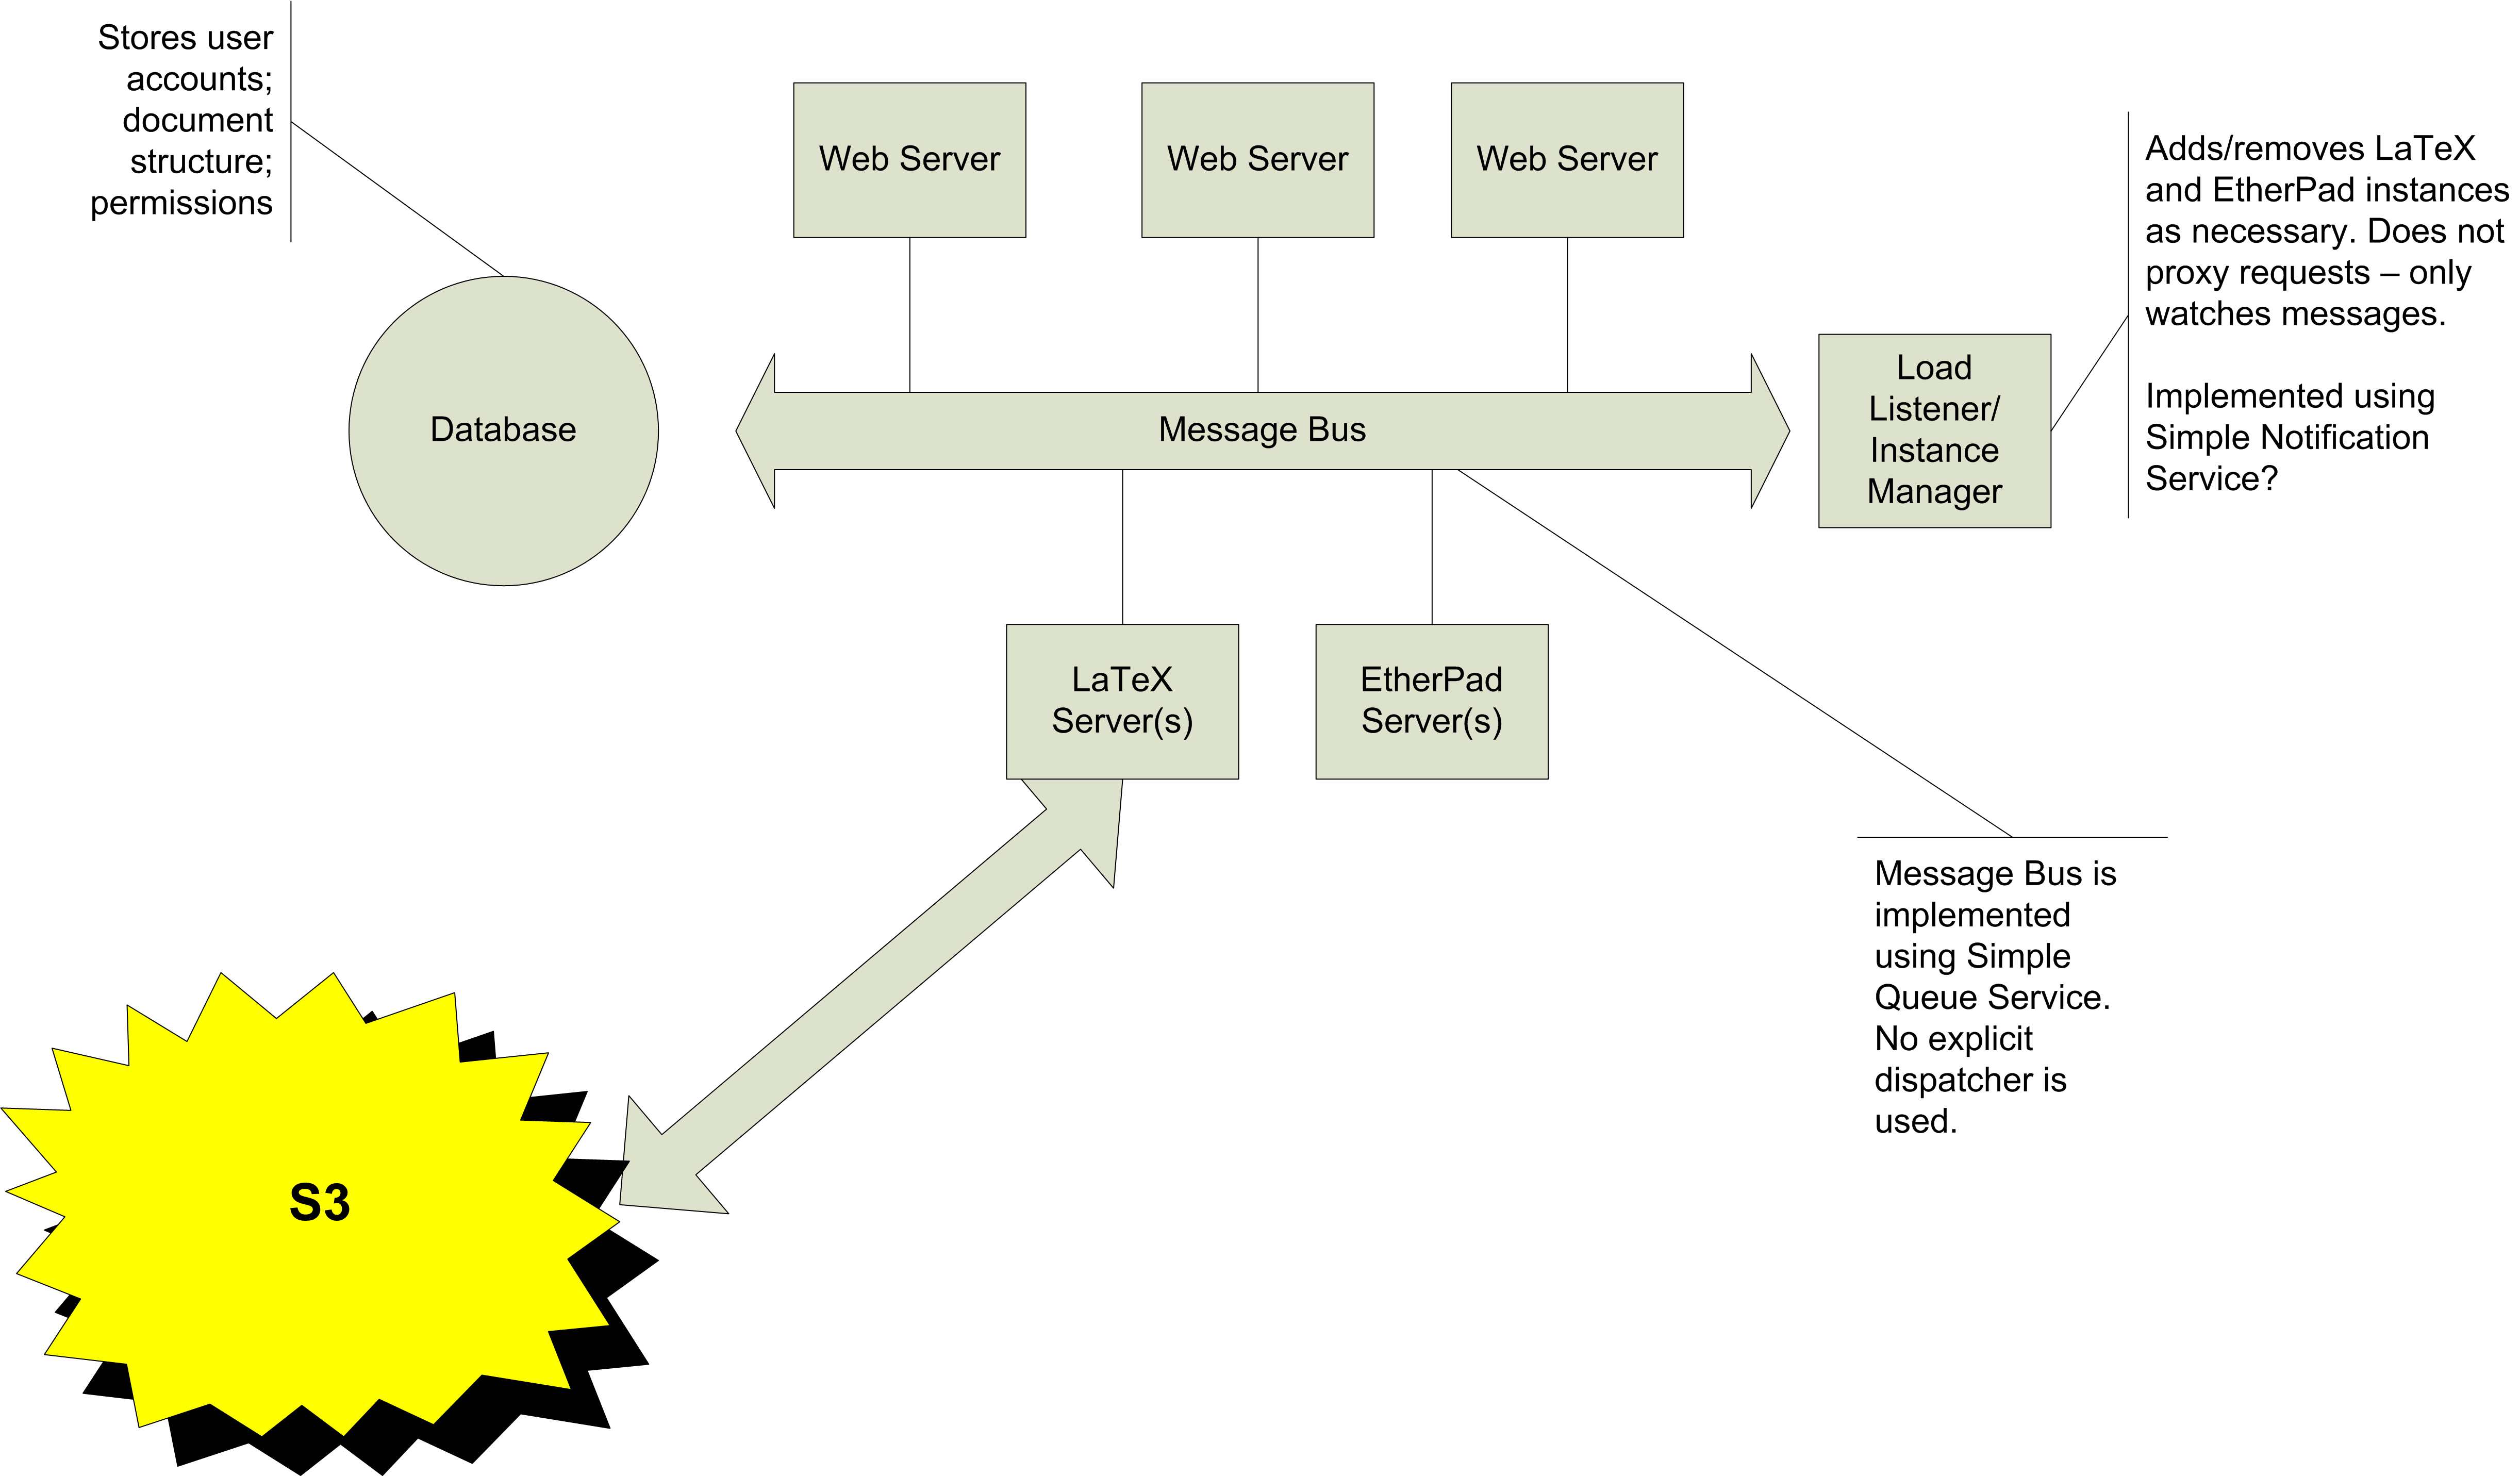
\includegraphics[width=6in,height=3.3738in]{SimpleTexArchitectureDiagram}
\caption{Initial sketch of the \STex architecture.}
\label{fig_arch}
\end{figure}

\end{document}
